\documentclass[11pt]{report}

\special{papersize=8.5in,11in}

\topmargin -0.5in \oddsidemargin 0.00in \evensidemargin 0.00in
\textwidth 6.75in \textheight 9.0in \headheight 0.25in \headsep
0.25in \footskip 0.5in \hoffset 0in \marginparpush 0.0in
\marginparwidth 0.0in \marginparsep 0.2in

\setcounter{page}{1}

\newcommand{\tabincell}[2]{\begin{tabular}{@{}#1@{}}#2\end{tabular}}  
\newcommand{\D}{\displaystyle}\newcommand{\T}{\textstyle}
\newcommand{\e}{{\mathrm{exp}}}
\newcommand{\dd}{{\mathrm d}}
\newcommand{\comment}[1]{}
\newcommand{\mb}{\mathbf}
\reversemarginpar

\usepackage[final]{graphicx}
\usepackage{fancyhdr}
%\graphicspath{{Papers/}}
\usepackage{amsthm,amssymb,amsmath}
\usepackage{cite}
\usepackage{geometry}
\usepackage{amsmath}
\usepackage{booktabs}
\usepackage{color}
\usepackage{setspace}
\usepackage{subfigure}
\usepackage{url}
\usepackage{multirow}
%\usepackage[top=2.5cm, bottom=2.5cm, right=3.5cm, left=3.5cm]{geometry}
\geometry{a4paper,scale=0.8}
\setcounter{secnumdepth}{3}

\title{Research Progress Report}

\author{Botao Zhu}

\begin{document}
	
	\maketitle
	\lhead{\sf Research Progress Report - 3rd} \chead{} \rhead{\sf Botao Zhu}
	\lfoot{CTRG, University of Saskatchewan} \cfoot{} \rfoot{Page \thepage}
	\renewcommand{\footrulewidth}{1.0pt}
	\renewcommand{\headrulewidth}{2.0pt}
	\renewcommand{\arraystretch}{1.3}
	\pagestyle{fancy}
	
	\renewcommand{\thesection}{\arabic{section}}
	
	\section{Reading and Research Activities}
	
	\subsection{Reading Summary}
	With the growth of network nodes and the expansion of application environment of WSNs, it needs to have the ability to handle huge network traffic and more flexibility. So, here are some main problems that need to be solved by Machine Learning.\\
	1) Because of  the changing rapidly of WSNs environments over time, it need to be adapted to these environments.\\
	2) For complicated network environments, a good mathematical model is needed to describe network behavior, which can reduce the complexity of WSNs problems.\\
	3) Relationship among network features, such as packet size, delay, error and path, are difficult to extract and describe.\\
	4) How to prolong the lifetime of WSNs by choosing the optimal path?\\
	
	\noindent Why machine learning is a good choice to solve these problems? Here is an example for routing search. Figure~\ref{1stafig} shows the original graph and Figure~\ref{1stbfig} is the traditional spanning tree routing. However, the routing problem can be divided into sub-problems by employing machine learning, shown in Figure~\ref{1stcfig}. Each node only needs to consider neighboring nodes' information  for deciding the optimal next node. 
	
	\begin{figure}[!h]
		\subfigure[]{
			\begin{minipage}[h]{0.3\linewidth}
				\centering
				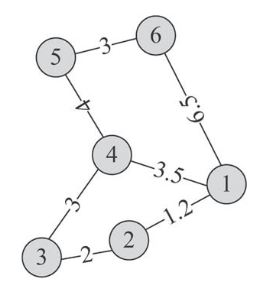
\includegraphics[width=2in]{figure1.jpg}
				\label{1stafig}
			\end{minipage}
		}%
		\subfigure[]{
			\begin{minipage}[h]{0.3\linewidth}
				\centering
				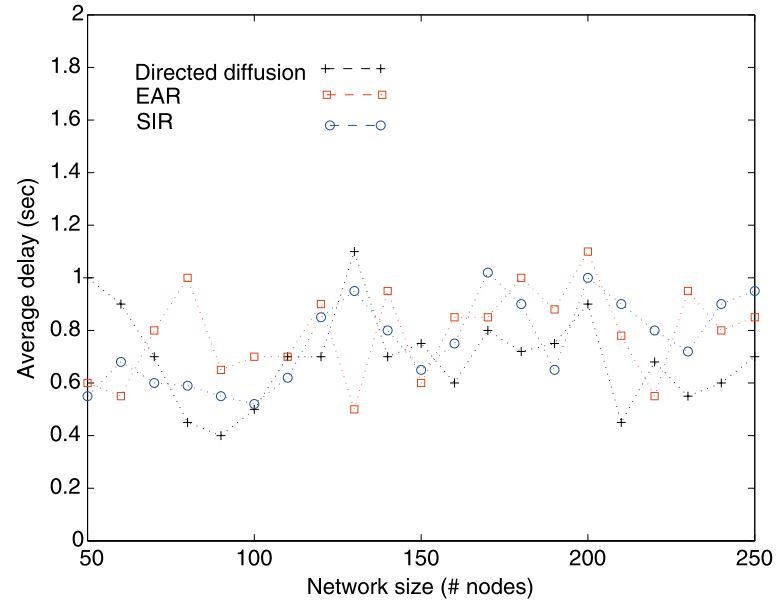
\includegraphics[width=2in]{figure2.jpg}
				\label{1stbfig}
			\end{minipage}
		}%
		\subfigure[]{  
			\begin{minipage}[h]{0.3\linewidth}
				\centering
				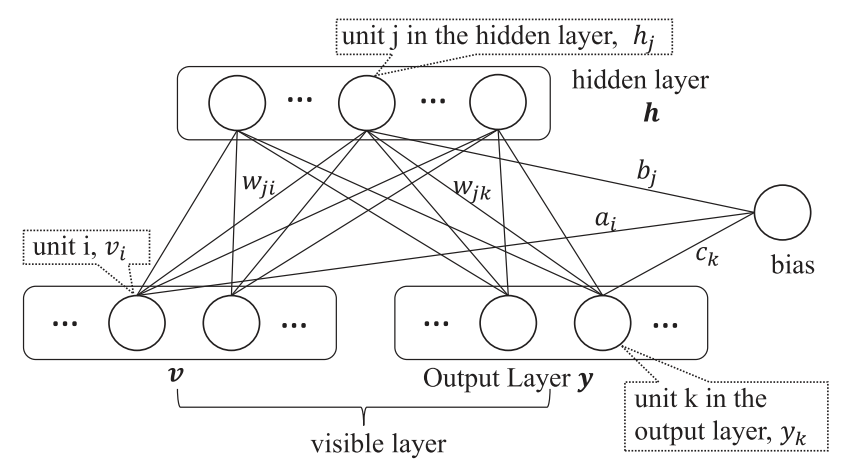
\includegraphics[width=2in]{figure3.jpg}
				\label{1stcfig}
			\end{minipage}
		}%
		\centering
		\caption{Example of routing problem}
	\end{figure}
	
	\begin{table}[!h]
		\centering
		\caption{Routing table of $R_3$}
		\begin{tabular}{c|c|c|c|c|c}
			\toprule
			Ref.& \tabincell{c}{Network\\ Simulation \\Tool} & ML Tool & Dataset Input & Dataset Output & Evaluation Index\\
			\hline
			\cite{06002} & Mininet\cite{mininet} & TensorFlow\cite{tensorflow} & \tabincell{c}{Network states \\+ traffic matrix} & optimal path & accuracy\\
			\hline
			\cite{4411037} & NS2 & NS2 & \tabincell{c}{location and \\energy of node \\and its neighbor} & next node & \tabincell{c}{packets sent, \\delivery ratio,\\average delay,\\network lifetime}\\
			\hline
			\cite{5408367} & Aqua-sim(NS2) & Aqua-sim(NS2) & \tabincell{c}{states set\\ actions set} & next node & \tabincell{c}{average latency \\ residual energy\\transmission errors\\ lifetime}\\
			\hline
			\cite{7792369} \cite{7935536} & C++ & WILL\cite{WILL} & traffic pattern & next node & \tabincell{c}{total throughput\\average per\\ -hop delay}\\ 
			\hline
			\cite{YangMinLee} & Qualnet 5.0 & word2vec & \tabincell{c}{node vector\\ message} & node degree & \tabincell{c}{packet delivery rate\\ route discovery time}\\
			\hline
			\cite{DBLP:journals/corr/abs-1709-07080} & OMNeT++ & not mentioned & \tabincell{c}{traffic matrix\\link weight} & mean of delay & transmission delay\\
			\hline
			\cite{DBLP:journals/corr/abs-1708-03074} & Not mentioned & CPLEX & traffic pattern & next node & \tabincell{c}{average congestion\\ratio  }\\
			\hline
			\cite{7791218} & NS2 & Not mentioned & \tabincell{c}{distance between\\each node \\and heads} & \tabincell{c}{position of\\cluster head} & energy dissipation\\
			\hline
			\cite{doi:10.1155/2015/618072} & NS2 & NS2 & \tabincell{c}{energy consumption\\transmit cost\\receive cost\\data packet size\\sensing radius} & \tabincell{c}{network lifetime\\ packet delivery\\ packet delay\\ network balance}\\
			\hline
		\end{tabular}
	\end{table}
	
	\noindent For the machine learning-based network topology, there are two main ideas: centralized model and distributed model. With regard to the centralized model, the advantage is that it uses the base stations with huge computation power to train machine learning model while the disadvantage is that the common network nodes are difficult to find the base stations in some cases, like the limitation of geography. However, in the distributed model, each node or edge router needs to train several machine learning models according to previous history network traffic for deciding next node. So, the main problems is each node needs to have the abilities of huge computation and storage. Specially, reinforcement learning and neural networks are the most commonly machine learning-based algorithms used in the distributed WSNs. Here is a brief summary.\\
	
	
	\begin{table}[!h]
		\centering
		\caption{}
		\begin{tabular}{c|c}
			\toprule
			ML Techniques & Ref.\\
			\hline
			Neural Network & \cite{7792369} \cite{7935536} \cite{8088549} \cite{8489985} \cite{8485423}\\
			\hline
			Reinforcement Learning & \cite{4411037} \cite{5408367} \cite{DBLP:journals/corr/abs-1709-07080} \cite{doi:10.1155/2015/618072}...\\
			\hline
		\end{tabular}
	\end{table}
     \noindent 1) Key steps of applying Neural Network in wireless networks\\     
     \noindent There are several steps that we need to consider for applying Neural network in wireless network.  
    \begin{itemize}
    	\item The extraction of traffic features matrix or vector\\
    	The input vectors is very important in training neural network. Because of the self-similarity of network traffic, we can use the previous network traffic characteristics to represent the later network traffic. How to choose the appropriate parameters to represent the relationship of network traffics is a very important issue. \cite{YangMinLee} creates a collection of 20-dimension vectors that can express a single feature in the node vector. \\
    	\begin{figure}[h!]
    		\centering
    		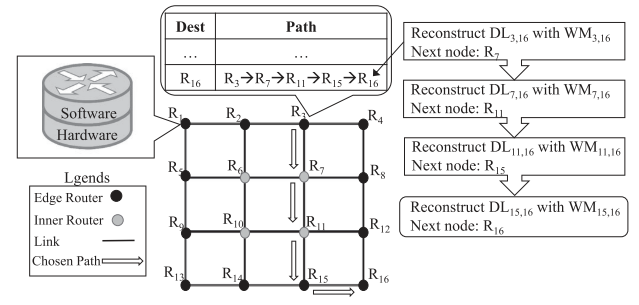
\includegraphics[width=0.9\linewidth]{figure4.jpg}
    		\caption{}
    		\label{2thfig}
    	\end{figure}\\
    \end{itemize}
	\begin{itemize}
		\item The design of neural network architecture\\
		There are different neural network models and it is important to choose which one.
		Normally, any neural networks comprise an input layer, multiple hidden layers and an output layer, shown in Figure~\ref{3thfig}. The input layer has N units which can be defined as the total number of nodes in the network. In the hidden layers, each layer can compute a non-linear transformation of the previous layer. The output of neural network is the routing path indicating the next router along the path from the source router to the destination. A N-dimensional vector can represent the output and each of its elements has a binary value. Only the position with value of 1 indicates the next node. 
		\begin{figure}[h!]
			\centering
			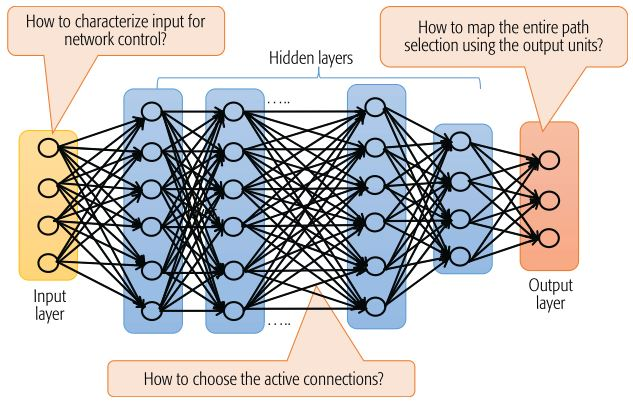
\includegraphics[width=0.7\linewidth]{figure5.jpg}
			\caption{Neural network architecture}
			\label{3thfig}
		\end{figure}\\
	\end{itemize}
	\begin{itemize}
		\item Routing search\\
		Assume there are 10 routers in the network, the source node is $n_1$, and the destination node is $n_10$. The first step of the running phase is to find the optimal router to the source. The NN model $NN_{1,10}$ is run by $n_1$. The input of $NN_{1,10}$ is vector $A=\left[\alpha_1, \alpha_2,\cdots, \alpha_10\right]$, where $\alpha_i$ is the traffic pattern of router $i$. At the output side, one out of 10 routers is chosen which is $n_3$ in the figure~\ref{4thfig}. Following that, node $n_1$ runs model $NN_{3,10}$ to find the second hop node. This operation is repeated until the destination node is reached.\\
		\begin{figure}[h!]
			\centering
			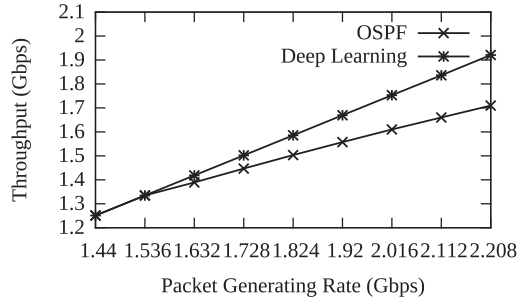
\includegraphics[width=0.6\linewidth]{figure6.jpg}
			\caption{Routing search}
			\label{4thfig}
		\end{figure}\\ 
	\end{itemize}
        
    \noindent In addition to the summary of the important parts above, there are other steps in the process of using neural network, such as initial phase, data collection and NN weight matrix update, etc. Here is a simple flow chart. For the detailed introduction of applying neural network into the field of routing search, please see ref. \cite{7792369}.
    \begin{figure}[h!]
    	\centering
    	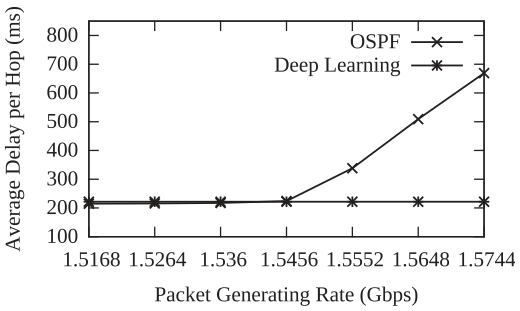
\includegraphics[width=0.6\linewidth]{figure7.jpg}
    	\caption{The flow chart of neural network based routing search method}
    	\label{5thfig}   
    \end{figure}\\ 
    
	\noindent By reading some literatures, only Professor N. Kato has done a lot of work in using neural network in the field of routing search. But his work assumes each node in the networks has the ability to train the neural network, which requires that each node has enough energy, storage capacity and computing capacity. At the same time, the neural network is supervised learning, how to obtain labeled data is also a big problem.
	
	
	
	
	
	
	
	
	In order to investigate the use of tools further, the following table lists the application of machine learning in other areas of networks.
	\begin{table}[!h]
		\centering
		\caption{Routing table of $R_3$}
		\begin{tabular}{c|c|c|c|c|c}
			\toprule
			& Ref.& \tabincell{c}{Network Simulation \\Tool} & ML Tool & Dataset Input & Dataset Output\\
			\hline
			\multirow{2}{*}{Name} & & & & \\ \cline{2-4}
		\end{tabular}
	\end{table}


	
	\subsection{Deep Learning Based Routing Strategy}
	\subsubsection{Input and Output Design}
	
	\subsubsection{Deep Learning Structure Design}
	The authors choose the DBA as the deep learning structures as shown in Figure~\ref{1stfig}.
	
	\subsubsection{The Procedures of the Proposed Deep Learning Based Routing Strategy}
	\paragraph{Initialization Phase}

	\paragraph{Training Phase}
              

	\paragraph{Running Phase}

	
	\subsubsection{Network Performance Analysis}
	They compared the proposed deep learning method with OSPF by the network signaling overhead, throughput and average delay. 
	
	\section{Objectives for the Next 2 Weeks}
	\subsection{Reading} 
	Reading papers foused on ML-based or DL-based routing.
	\subsection{Course} 
	Studying chapter 1 and chapter 2 of Neural Networks and Deep Learning, \textbf{Coursera}. \url{https://www.coursera.org/learn/neural-networks-deep-learning}
	\subsection{Code}
	Studying the classic routing protocol: LEACH and using Matlab to implement.
	
	\section{Advisor's Comments}
	
	\bibliographystyle{IEEEtran}
	\bibliography{janbib}
	
\end{document}